\documentclass[aspectratio=169]{beamer}
\usepackage{amsmath}
\usepackage{amssymb}
\usepackage{amsfonts}
\usepackage{graphicx}
\usepackage{luatexja} 
\usepackage{comment}
\usepackage{bm}
\usepackage{setspace}
\usepackage{caption}

\usetheme{LightTheme}
\setbeamertemplate{footline}[frame number]
\setbeamertemplate{navigation symbols}{}
\setlength{\baselineskip}{10pt}
\begin{document}

% タイトルフレーム
\title{進捗状況}
\subtitle{React\ Hook} 
\author{\small B4 小林紹子} % 必要に応じて変更・削除
\date{\small\today} % 必要に応じて変更・削除

\begin{frame}
    \titlepage
\end{frame}

\begin{frame}{目次}
    \tableofcontents
\end{frame}

\section{React\ Hook}

\begin{frame}{useCallback}
    \begin{itemize}
        \setlength{\itemsep}{2em}
        \item useCallbackは関数をメモ化するためのフック.
        \item useCallbackの第一引数は関数で,第二引数は依存配列.
        \item 関数の再描画が行われる際に,useCallback()は依存配列の中の値を比較.
        \item 依存配列の値がそれぞれ同じ場合は,useCallback()はメモ化している関数を返す.
        \item 異なる場合は,現在の第一引数の関数をメモに保存する.\rightarrowfill 新しい関数を返す.
    \end{itemize}
\end{frame}

\begin{frame}{memo関数とuseCallbackの関係}
    \begin{itemize}
        \setlength{\itemsep}{2em}
        \item memo関数
        \begin{itemize}
            \item propsが同じであれば再描画をスキップする.
        \end{itemize}
        \item useCallback
        \begin{itemize}
            \item 関数の参照をメモ化.
            \item 依存配列が変わらない限り,同じ関数オブジェクトを再利用.
            \item 再レンダーされても「新しい関数が作られる」ことはない.
        \end{itemize}
    \end{itemize} 
    \rightarrowfill useCallbackとmemo関数を同時に使うことで再描画を防げる.

\end{frame}
\begin{frame}
    \begin{figure}
        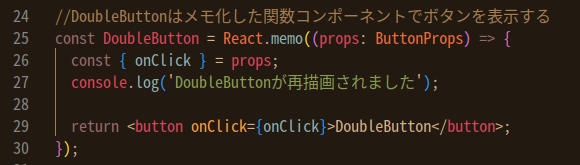
\includegraphics[scale = 0.5]{useCallback1.png}
    \end{figure}
    \begin{figure}
        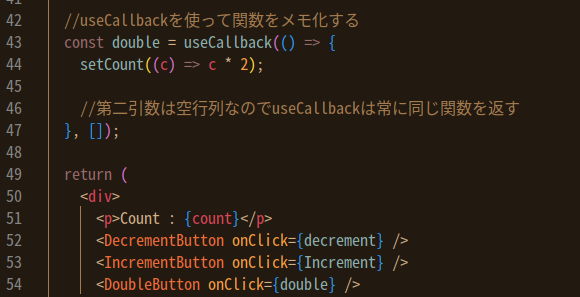
\includegraphics[scale = 0.5]{useCallback2.png}
    \end{figure}
\end{frame}

\section{Next.jsとReact}

\begin{frame}[allowframebreaks]{Next.jsとReact}
    \begin{itemize}
        \setlength{\itemsep}{2em}
        \item Next.js : Reactをベースに開発されたフレームワーク.
        \item React : Javascriptにおけるライブラリの一つ.
    \end{itemize}
    \vspace{2em}
    ライブラリ:\\開発時に使われるコードの集まり.作業を簡略化するための関数や定義・クラスの集まり.\\
    フレームワーク:\\テンプレートのようなもの.ログイン機能や決算機能など必要な機能がデフォルトで揃っている.\\
    \Rightarrow Next.jsはReactライブラリのフレームワーク
    \begin{figure}
        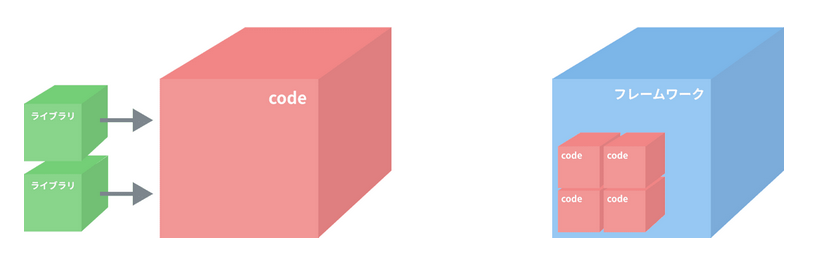
\includegraphics[scale=0.5]{Next.js_and_React.png}
        \caption{ReactとNext.js}
    \end{figure}
\end{frame}

\begin{frame}[allowframebreaks]{Next.jsの特徴}
    \begin{itemize}
        \item RCS(React Server Components)
        \begin{itemize}
             \setlength{\itemsep}{2em}
            \item Reactは従来SSR(Server Side Rendering)を行ってきた.
            \item SSR : 全てのコンポーネントをサーバーでHTMLに変換する.
            \item RCSでは、それをサーバーで実行する部分とクライアントで実行する部分を分けることができる.
            \item これにより,無駄なリロードが減る.
        \end{itemize}
        \newpage
        \item App Router
        \begin{itemize}
            \item ディレクトリ構造がそのままURLの構造になる.
            \item ルーティングは/app配下のディレクトリベースで行う.
            \item page.tsxでルートの画面,router.tsxでAPIエンドポイントを書くなどファイル規約がある.
            \begin{figure}
                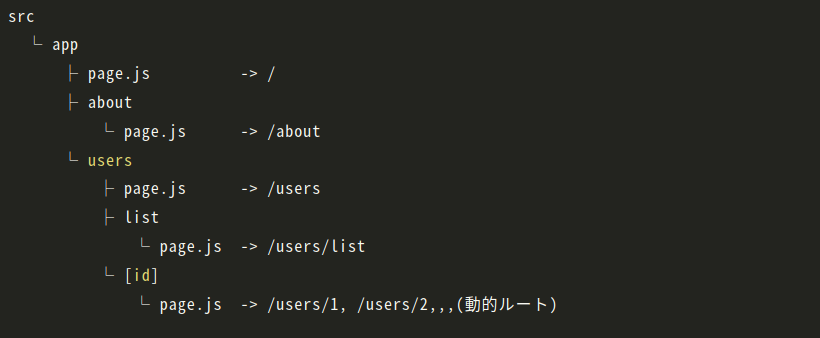
\includegraphics[scale=0.35]{AppRouter.png}
            \end{figure}
        \end{itemize}
    \end{itemize}
\end{frame}

\section{作業経過}
\begin{frame}{環境構築}
    \begin{itemize}
        \setlength{\itemsep}{1em}
        \item npmをインストール(sudo apt npm)version : v22.15.0
        \item Next.jsをインストール(npx create-next-app@latest --ts next-sample)version:v22.15.0
        \item ここでTurbopackが開発サーバークラッシュしてるとエラーがでた.
        \item \rightarrow nodemoduleとpackage.jsonを削除
        \item npm i で再インストールするとうまくいった.
        \item npm run devで初期画面がでてきた.(http://localhost:3000)
    \end{itemize}    
\end{frame}

\begin{frame}{画面描画}
    \begin{itemize}
        \setlength{\itemsep}{2em}
        \item React Flow : インタラクティブなダイアグラムを簡単に実装できる.
        \item npm install reactflow
        \item 作れはしたが、もともとチャートフロウなどを書く用に作られたものだったので上手な図形は作れず.
    \end{itemize}
\end{frame}

\begin{frame}[allowframebreaks]{コード}
    \begin{figure}
        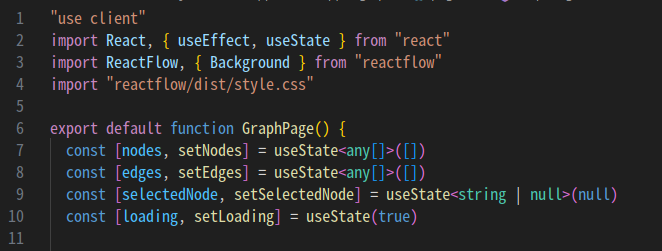
\includegraphics[scale=0.6]{graph1.png}
        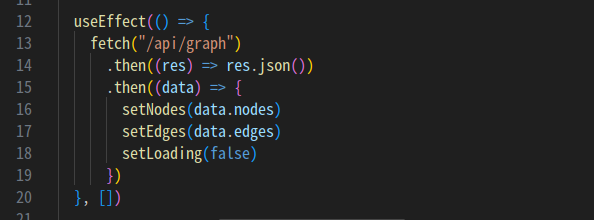
\includegraphics[scale=0.6]{graph2.png}
    \end{figure}
\end{frame}

\begin{frame}{○×問題}
    \begin{itemize}
        \setlength{\itemsep}{2em}
        \item まずはバックエンド・フロントエンドに問題・回答を書いた.
        \item JSONで答えをサーバからもらって判断する.
        \item 将来的にはデータベースから問題を取得するようにする.
    \end{itemize}
\end{frame}

\begin{frame}[allowframebreaks]{フロントエンド(page.tsx)}
    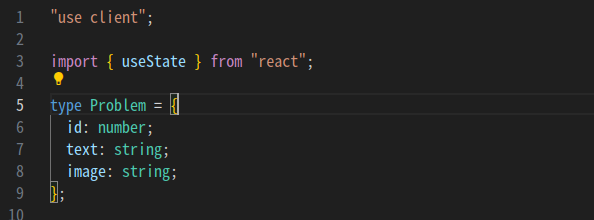
\includegraphics[scale=0.6]{q1.png}
    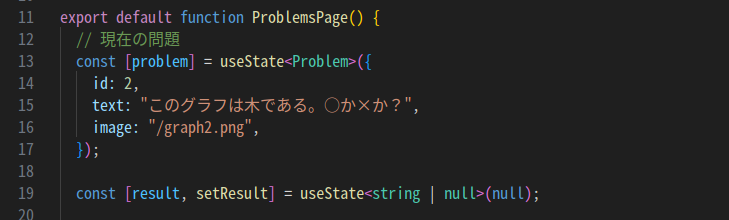
\includegraphics[scale=0.6]{q2.png}
    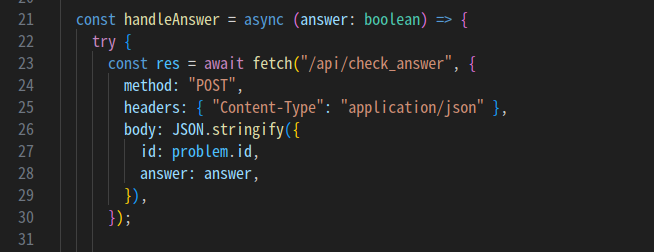
\includegraphics[scale=0.6]{q3.png}
    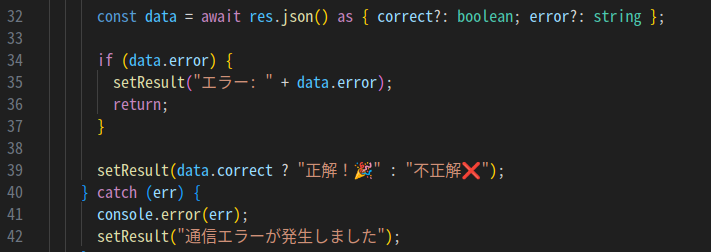
\includegraphics[scale=0.6]{q4.png}
\end{frame}

\begin{frame}[allowframebreaks]{バックエンド(route.tsx)}
    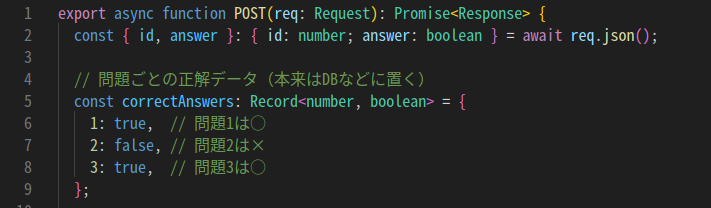
\includegraphics[scale=0.6]{check1.png}
    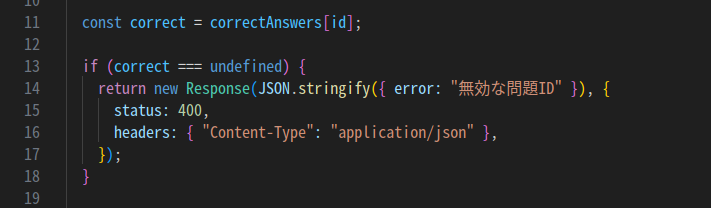
\includegraphics[scale=0.6]{check2.png}
    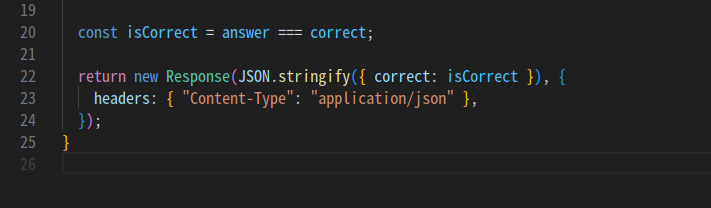
\includegraphics[scale=0.6]{check3.png}
\end{frame}
\end{document}


